%!TEX root = ../main.tex

In practically interesting Bayesian models, the posterior distribution is often computationally intractable to obtain and therefore one has to resort to approximate inference techniques. The most popular approximation methods are variational inference and Markov chain Monte Carlo.

Variational methods operate by minimising an information theoretic divergence between a simple distribution, often of exponential family, and the true posterior. The divergence is often chosen to be a form of Kullback-Leibler divergence, as it allows easy rearrangement of terms and makes local message-passing style computations possible. In section \ref{sec:losscalibrated} argue that when Bayesian inference is performed to solve a particular decision problem, these algorithms are sub-optimal as they are ignorant of the structure of losses. We devised a framework we termed loss-calibrated approximate inference \cite{}, which generalises traditional variational approaches by minimising generalised divergences based on scoring rules. I will demonstrate this framework on a loss-critical toy problem and on a well-known nonparametric Bayesian model, Gaussian process regression.

Monte Carlo methods produce random samples (approximately) drawn from the posterior, which then allow for approximating relevant integrals over the posterior. Monte Carlo techniques are applicable to a wide variety of interesting Bayesian models, and allow for an intuitive trade-off between computation time and accuracy. However, just as most variational approaches, Monte Carlo techniques are also ignorant of the decisions and losses involved in a decision problem. In section \ref{sec:} I introduce a new class of approximate inference algorithms that I call loss-calibrated quasi-Monte Carlo methods. These algorithms produce a deterministic sequence of pseudo-samples in such a way, that the divergence between the empirical distribution of pseudosamples is minimised from the target distribution. I show how kernel herding, a recent algorithm proposed by \cite{kernelherding} can be seen as a special case of loss-calibrated quasi-Monte Carlo, and point out the connection between this method and Bayesian Quadrature.

The work presented in this chapter on loss-calibrated approximate inference and approximate decision theory is joint work with Simon Lacoste-Julien and Zoubin Ghahramani, and most of the results presented here have been published in \cite{losscalibrated}.
The work presented on the equivalence between optimally weighted kernel herding and Bayesian Quadrature is joint work with David Duvenaud, and has been published \cite{losscalibrated}.

\section{Loss-calibrated approximate inference}

\TODO{General paragraph about Bayesian inference}

In many practically relevant cases computing the posterior is not analytically tractable. This is predominantly due to the fact that the integral defining the marginal likelihood $\int p(\dataset\vert\theta)p(\theta)d\theta$ cannot be computed analytically in closed form, and therefore the normalisation of the posterior cannot be computed. But sometimes the complexity of evaluating even the unnormalised posterior increases exponentially with the amount of observed data, as in the case of for example switching state space models. In either case, it is usual practice to approximate the intractable posterior by something simpler, an approximate distribution $q$. The problem of finding an approximate posterior $q$ is referred to as approximate inference.

Over the years, two dominant branches of approximate inference emerged. The first branch, that I will refer to as parametric approximation schemes, includes variational inference, Laplace approximation and expectation propagation. The common theme in these techniques is that the complicated posterior is replaced by an approximate distribution chosen from a particular parametric family of distributions, usually from an exponential family. These methods differ in their objective functions they minimise, which measure discrepancy between the target posterior distribution and the approximation $q$.

\subsection{Overview of variational methods and expectation propagation}

Variational methods to approximate inference find the optimal approximation $q^{*}$ to the posterior by maximising a lower bound to the marginal likelihood as follows.

\begin{align}
	\log p(\dataset) &= \log \int p(\dataset\vert\theta)p(\theta) d\theta\\
		&=\log \int \frac{p(\dataset\vert\theta)p(\theta)}{q(\theta)}q(\theta) d\theta\\
		&\geq \int \log \frac{p(\dataset\vert\theta)p(\theta)}{q(\theta)} q(\theta) d\theta\\
		&= \log p(\dataset) - \KL{p_{\dataset}}{q}
\end{align}

by minimising the Kullback-Leibler divergence (Eqn.\ \eqref{eqn:KL_divergence}) between the approximate distribution $q$ and the true posterior $p_{\dataset}$. A common practice in approximate inference is to choose the approximate posterior distribution $q$ from an exponential family of distributions $\Qe$, and it is also often common practice to choose $q$ such that it factorises over multivariate quantities. When these assumptions are made, the solution to the above optimisation can often be expressed in closed form, or efficient iterative algorithms exist for finding a locally optimal solution numerically.

The KL divergence is non-symmetric, therefore the order of arguments matter. Variational methods minimise $\KL{q}{p_{\dataset}}$, that is with the approximate distribution being the first argument. On the one hand, this is highly convenient as computing the divergence in this direction requires integration only over $q$, which is assumed simpler than the real posterior $p_{\dataset}$.On the other hand, as I argued in section \ref{sec:scoring_rules}, in the scoring rule interpretation suggests that the \emph{right} way to use divergence is $\KL{p_{\dataset}}{q}$, i.\,e.\ when its first argument is the true distribution we want to approximate, and the second argument some approximation $q$. This has been pointed out previously by \cite{Csato2002,Minka2001} and many other authors. This does not mean that variational inference does not work, it just means that by performing variational inference we loose some of the intuitive interpretation of KL divergence as Bregman divergence under the logarithmic loss.

Several approaches therefore tried to fix this conceptual issue, and minimise KL divergence in the opposite direction. This is unfortunately a challenge, as computing the divergence $\divergence{\score}{p_{\dataset}}{q}$ always requires an integral over the posterior $p_{\dataset}$, which is normally intractable, and this is why we perform approximate inference in the first place.

Assumed density filtering, and its generalisation, expectation propagation (EP) try to approximate the ideal method of minimising $\KL{p_{\dataset}}{q}$ as follows. EP assumes the posterior can be written as a product of factors as such:

\begin{equation}
	p_{\dataset}(\theta) = \frac{1}{Z} \prod t_i(\theta)
\end{equation}

The terms $t_i$ are assumed simple, and in most cases depend only on a few components of the multivariate parameter vector $\theta$. What makes the posterior intractable is the normalisation constant $Z$, computing which would involve a very expensive integral. Expectation propagation approximates the posterior by substituting approximate factors $\tilde{t}_i$ for original factors $t_i$, in such a way that the product of approximate factors

\begin{equation}
	q(\theta) = \prod \tilde{t}_i(\theta)
\end{equation}

is tractable. The approximate factors are improved one-by-one using the following objective function:

\begin{equation}
	\tilde{t}_i^{new} = \argmin_{t \in \text{approximate family}} \KL{\frac{1}{\int q(\theta)\frac{t_i(\theta)}{\tilde{t}_i(\theta)} d\theta}q(\theta)\frac{t_i(\theta)}{\tilde{t}_i(\theta)}}{q(\theta)\frac{t_i(\theta)}{t(\theta)}}
\end{equation}

Essentially, in each iteration the algorithm replaces one of the approximate factors in the approximate posterior $q$ with the real factor to construct a one-step-closer-to-exact approximation to the posterior $\tilde{q}$. Then it uses this $\tilde{q}$ as the target distribution and computes a new approximation by minimising KL divergence. This step is repeated until convergence, that is until no approximate factors can be further improved by the KL divergence metric.

Thus in expectation-propagation, the KL divergence is used in the right direction that is well motivated by the theory of scoring rules and Bregman divergences. However, as computing KL divergence in the right direction is intractable it has to use a roundabout method.

\subsection{Loss-calibrated approximate inference}

Although often overlooked, the main theoretical motivations for the Bayesian paradigm are rooted in Bayesian decision theory~\cite{berger85decision}, which provides a well-defined theoretical framework for rational decision making under uncertainty about a hidden parameter $\theta$. Approximate inference is concerned with approximating the posterior, but often ignores the fact that the posterior is then used in a wider context to make optimal decisions. In this section I review the theory of Bayesian decisions, and then devise a framework for addressing questions that arise when using approximate inference in the context of optimal decision making.

The ingredients of Bayesian decision theory are (see Ch.~2 of~\cite{robert01choice} or Ch.~1 of~\cite{berger85decision} for example):
\vspace{-.3cm}
\begin{itemize}
  \item a loss $\loss(\theta,\action)$ which quantifies the cost of taking action $\action \in \actionset$ when the world state is $\theta \in \Theta$; %\footnote{Note that $\theta$ is not assumed to be finite dimensional; in the most general setting, it could fully specify an arbitrary distribution over $\mathcal{O}$.};
  \item an observation model $p(\dataset|\theta)$ which gives the probability of observing some data or dataset $\dataset \in \mathcal{O}$ assuming that the world state is $\theta$;
  \item a prior belief $p(\theta)$ over world states.
\end{itemize}

The loss $\loss$ describes the decision task that we are interested in, whereas the observation model and the prior represent our beliefs about the world. Given these components, the ultimate objective for evaluating a possible action $\action$ after observing $\dataset$ is the \emph{expected posterior loss} (also called the \emph{posterior risk}~\cite{schervish95theory})

\begin{equation}
	\risk_{p_\dataset}(\action) \doteq \int_\Theta \loss(\theta, a) \, p(\theta|\dataset) d\theta
\end{equation}

In the Bayesian framework, the optimal action $\action_{p_\dataset}$ is the one that minimizes $\risk_{p_\dataset}$.

In this framework it is therefore easy to see that Bayesian decision making decomposes into two consecutive steps of computation. First, a posterior $p_\dataset$ is inferred from observed data $\dataset$, then the optimal action is selected by minimising risk under this posterior. Crucially, the first step is independent of losses, the posterior can be computed irrespective of how the loss $\loss$ is defined. In fact, once we have computed the posterior, the same distribution can be used to solve different decision problems with different losses involved. This independent breakdown of computation is what makes the posterior distribution such an important object in Bayesian statistics.

But when the posterior is intractable to compute and approximations are needed - as it is the case most of the time - additional questions arise. Is this two-step breakdown of computations to inference and then risk minimisation still a sensible thing to do? How should we decide what approximate inference method to use? Can we still re-use the same approximate posterior with different loss functions just as we can if no approximations are needed. Is the choice of approximate inference technique independent of the loss function? This chapter introduces loss-calibrated approximate Bayesian inference is a theoretical framework for addressing these questions.

To illustrate the role and behaviour ot approximate inference in a Bayesian decision problem consider the following simple problem. Suppose that we control a nuclear power-plant which has an unknown temperature $\theta$ that we model with Bayesian inference based on some measurements $\mathcal{D}$.
The plant is in danger of over-heating, and as the operator, we can take two actions: either shut it down or keep it running. Keeping it running while the temperature is above a critical threshold $T_\mathrm{crit}$ will cause a nuclear meltdown, incurring a large loss $L(\theta>T_\mathrm{crit},\mbox{'on'})$. On the other hand, shutting down the power plant incurs a moderate loss $L(\mbox{'off'})$, irrespective of the temperature. 
%Given our posterior $p_\dataset$ and the losses, we want to compute the Bayes-optimal action that minimizes the posterior risk. 
Suppose that our current observations yielded a complicated multi-modal posterior $p_\dataset(\theta)$ (\ref{fig:toy}, solid curve) that we do not have comutational resources to represent. Thus we chose to approximate it with a simple Gaussian distribution.

Now consider how various approaches to approximate inference would perform in terms of their Bayesian posterior risk. Minimizing $\KL{q}{p_\dataset}$, as in variational inference, yields candidate $q_1$ which concentrates around the largest mode, ignoring entirely the second small mode around the critical temperature \ref{fig:toy}, dotted curve). Minimizing $\KL{p_\dataset}{q}$ gives a more global approximation: $q_2$ matches moments of the posterior, but still underestimates the probability of the temperature being above $T_\mathrm{crit}$, thereby leading to a suboptimal decision \ref{fig:toy}, dashed curve).

\TODO{Rewrite as divergences have not been definded yet} $q_3$ is one of the minimizers of $d_L(p_\dataset \| q)$ in this setting, resulting in the same decision as $p_\dataset$ \ref{fig:toy}, dash-dotted curve). Note that $q_3$ does not model all aspects of the posterior, but it estimates the Bayes-decision well. Because there are only two possible actions in this setup, the set $\mathcal{Q}$ is split in only two halves by the function $d_L(p_\dataset,q)$ and so there are infinitely many $q_\mathrm{opt}$'s that are equivalent in terms of their risk. In contrast, in the predictive setting of section~\ref{ss:predictive} where in addition we assume $\mathcal{X}$ and $p(x)$ to be continuous, we could obtain a finer resolution $d_L(p_\dataset \| q)$ which can potentially yield a unique optimizer.

This simple example already highlighted some features of the loss-calibrated framework. First of all, it is clear, that even in a simple example the choice of approximate inference methods matters, and has a great influence on risks and the final decisions made. In this case minimising $\KL{p_\dataset}{q}$ yielded a solution superior to minimising the variational criterion $\KL{q}{p_\dataset}$, but we could just as well construct another example, where it is the other way around. Even though $\KL{p_\dataset}{q}$ is thought of as the more principled method, in the context of this decision problem neither of them is clearly better or more principled than the other.

\subsection{The loss-calibrated approximate inference framework}

In practice, one usually treats the approximate $q$ as if it was the true posterior and chooses the action that minimizes what we will call the \emph{$q$-risk}:
\begin{equation} \label{e:q-risk}
    \mathcal{R}_q(h) \doteq \int_\Theta q(\theta) L(\theta,h) d\theta ,
\end{equation}
obtaining a \emph{$q$-optimal} action $h_q$:
\begin{equation}
    h_q \doteq \argmin{h \in \mathcal{H}} \mathcal{R}_q(h).
\end{equation}
In this paper, we will assume that computing exactly the $q$-optimal action $h_q$ for $q \in \mathcal{Q}$ is tractable, and focus on the problem of choosing a suitable $q$ to approximate the posterior $p_\dataset$ \emph{in order to yield a decision $h_q$ with low posterior risk $\mathcal{R}_{p_\dataset}(h_q)$}, mimicking the standard methodology but crystallizing the decision theoretic goal. Given this approach, a (usually non-unique) optimal $q \in \mathcal{Q}$ is clearly:
\begin{equation}
    q_\mathrm{opt} = \argmin{q \in \mathcal{Q}} \mathcal{R}_{p_\dataset}(h_q),
\end{equation}
though a practical algorithm might only be able to find an approximate minimizer to this quantity. In the case where $p_\dataset\in\mathcal{Q}$, $p_\dataset$ is obviously optimal according to this criterion.

We could interpret the above criterion as minimizing the following asymmetric non-negative discrepancy measure between distributions:
\begin{equation} \label{e:d_L}
    d_L(p\|q) \doteq \mathcal{R}_{p}(h_q) - \mathcal{R}_{p}(h_p).
\end{equation}
Interestingly, the Kullback-Leibler divergence $KL(p\|q)$ can be interpreted as a special case of $d_L$ for the task of posterior density estimation over $\Theta$. In this task, an action $h$ is a density over $\Theta$ and the standard density estimation statistical loss is $L(\theta,h) = -\log h(\theta)$. The $q$-risk $R_q(h)$ then becomes the cross-entropy $H(q,h)=-\int_\Theta q(\theta) \log(h(\theta)) d\theta$, and so $h_q = q$ assuming that $q \in \mathcal{H}$. Under these assumptions, we obtain that $KL(p\|q) = d_L(p\|q)$ and so as was already known in statistics, $KL(p_\dataset\|\cdot)$ appears ``loss-calibrated'' for the task of posterior density estimation in our approximation framework. But this begs the natural question of whether minimizing $d_L$ for a particular loss $L$ provides optimal performance under other losses. We will show in \ref{ss:GPR} that even in the simple Gaussian linear regression setting, minimizing the KL divergence can be suboptimal in the squared loss sense, thus motivating us to seek loss-calibrated alternatives.

\paragraph{Example: Gaussian process regression}

In this case we do not actually need to perform approximate inference, as the posterior is Gaussian and available in closed form. However it allows us to express the quantities relevant for loss-calibrated approximate inference.
§
Gaussian process regression.

\section{Loss-calibrated quasi-Monte-Carlo}

\paragraph{Monte Carlo - about two paragraphs}
A popular alternative to parametric approximation schemes, such as variational inference and expectation propagation are Monte Carlo methods.

Monte Carlo methods produce random samples from the posterior distribution $p_\dataset$ and then approximate relevant integrals by taking the empirical means over these samples. Subject to smoothness conditions, this non-deterministic estimate of any integral converges at a rate $\mathcal{O}(\frac{1}{\sqrt{N}})$, where $N$ is the number of samples. This convergence is guaranteed by the law of large numbers. An appealing property of Monte Carlo methods is that in theory an arbitrarily precise estimate can be obtained by just increasing the number of samples. In this sense, Monte Carlo approximation is non-parametric: the number of parameters that describe the approximate distribution is not fixed ahead of time, and can be arbitrarily large.

When exact sampling from $p_\dataset$ is impossible or impractical, Markov chain Monte Carlo (MCMC) methods are often used. MCMC methods only require knowing the target distribution up to a constant factor. Practically this means that even if the normalisation constant of the posterior is intractable, MCMC techniques can still be used to generate samples from it.

Various variants of MCMC methods can be applied to almost any problem but the convergence rate of the estimate depends on several factors and is hard to estimate \citep{CowlesCarlin96}. Typically, MCMC techniques introduce positive correlation between subsequent samples, and thus are less effective than exact Monte Carlo sampling. For an overview of various Monte Carlo techiques, see \citep{Murray2007}.

Monte Carlo methods are very general, they guarantee convergence for any measurable integral. Hence, convergence is also guaranteed in the KL divergence sense, and as the posterior risk is expressed as an integral, they also ensure convergence in $d_\loss(\cdot\|\cdot)$ for any loss function $\ell$. However, the rate of convergence cannot be fine-tuned to a particular divergence measure. One might hope that if the loss function $\ell$ is known ahead of time, a faster convergence rate can be achieved, maybe at the cost of slowing down convergence on integrals that are irrelevant to the decision problem.

\paragraph{revisit toy example} Let us consider the power plant example from the previous section. To be able to make a decision, the only thing we need to know is the probability of the temperature exceeding the critical temperature. Thus, when the distribution is approximated via Monte Carlo, the only summary statistic we care about is the fraction of samples that are above the critical temperature.

The probability of interest can be written as the expectation of the indicator function that takes value $1$ if the temperature exceeds the critical one and $0$ otherwise. This indicator function is measurable, therefore an $\mathcal{O}(\frac{1}{\sqrt{N}})$ convergence is guaranteed by exact MCMC sampling.
However, it is easy to construct an ideal series of $N$ `pseudo-samples' where the error is upper bounded by $\frac{1}{N}$. (The problem is equivalent to approximating the probability with a series of rational numbers). This ideal set of $N$ pseudosamples may of course be a terrible general approximation to the full probability distribution $p_\dataset$, but from the perspective of the decision problem it converges much faster than the random Monte Carlo samples.

\TODO{illustrate this on figures: Fig 1: same as in previous section. Fig 2: approximating the probability with random MCMC and with optimal QMC}

\paragraph{Quasi monte Carlo approaches}

 The focus of this chapter are quasi-Monte Carlo methods that -- instead of sampling randomly -- produce a set of pseudo-samples in a deterministic fashion. These methods operate by directly minimising some sort of discrepancy between the empirical distribution of pseudo-samples and the target distribution. Whenever these methods are applicable, they achieve convergence rates superior to the $\mathcal{O}(\frac{1}{\sqrt{N}})$ rate typical of random sampling.

TODO{review existing quasi-Monte-Carlo methods: Sobol sequences, Halton sequence}

The quasi-Monte-Carlo methods reviewed here often achieve faster convergence rates than traditional random Monte Carlo, but they are general-purpose sampling tools: they cannot be fine-tuned to particular decision problems we may want to use them for. Here I will introduce a class of quasi-Monte-Carlo methods that I will call loss-calibrated QMC. 

Quasi-Monte-Carlo can be interpreted as a special case of approximate inference, where the approximating family is the family of empirical distributions
\begin{equation}
	q(x ; x_1,\ldots,x_N) = \frac{1}{N} \sum_{n=1}^{N} \delta(x - x_n)\mbox{,}
\end{equation}
or weighted empirical distributions
\begin{equation}
	q(x ; x_1,\ldots,x_N,w_1,\ldots,w_N) = \sum_{n=1}^{N} w_n \delta(x - x_n)\mbox{.}
\end{equation}

Finding the optimal loss-calibrated sample set can then be achieved by minimising the loss-calibrated divergence $d_\loss$ between the target distribution $p_\dataset$ and the approximation $q$:

\begin{equation}
	\{x_1,\ldots,x_N\}_{n=1}^{N} = \argmin_{\{x_1,\ldots,x_N\}_{n=1}^{N}} \divergence{\loss}{p_\dataset}{q(x ; x_1,\ldots,x_N)} \label{eqn:loss_calibrated_nonsequential}
\end{equation}
It is important to note, that the above procedure does not make sense for general Bregman divergences. For example, the KL divergence $\KL{p}{q}$ requires the approximate distribution $q$ to be absolutely continuous with respect to the target distribution $p$, which, unless the target distribution is also discrete, cannot be satisfied if $q$ is atomic.

The minimisation in Equation \eqref{eqn:loss_calibrated_nonsequential} is 
\paragraph{Myopic sequential loss-calibrated Quasi Monte Carlo}


In most cases - just as loss-calibrated approximate inference in general, algorithmic implementations of loss-calibrated QMC requires the ability to evaluate certain integrals over the target distribution easily, therefore practical applications of loss-calibrated QMC in the form presented here are limited. Nevertheles, the framework may provide useful blueprint for designing sampling algotithms that are more tailored to particular decision scenarios.

%!TEX root = ../main.tex
\definecolor{mydarkblue}{rgb}{0,0.08,0.45}

\begin{figure}[h]
\centering
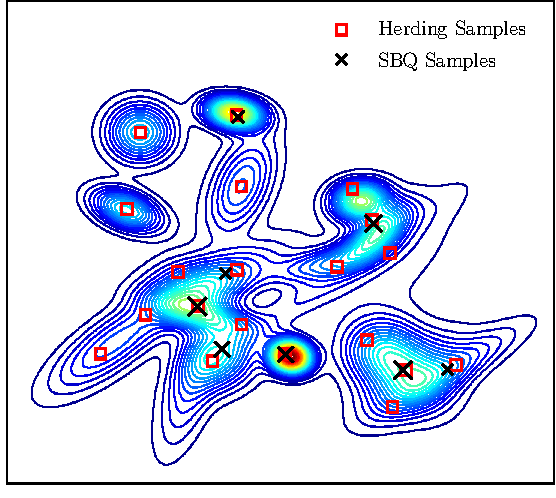
\includegraphics[width=\columnwidth]{figs/herding/fig1_v2}
\caption{The first 8 samples from sequential Bayesian quadrature, versus the first 20 samples from herding.  Only 8 weighted \sbq{} samples are needed to give an estimator with the same maximum mean discrepancy as using 20 herding samples with uniform weights.  Relative sizes of samples indicate their relative weights.}
\label{fig:fig1}
\end{figure} 

\subsubsection{INTRODUCTION}
\paragraph{The problem: Integrals} A common problem in statistical machine learning is to compute expectations of functions over probability distributions of the form:
\begin{equation}
	Z_{f,p} = \int f(x) p(x) dx \label{eqn:integral}
\end{equation}
Examples include computing marginal distributions, making predictions marginalizing over parameters, or computing the Bayes risk in a decision problem. In this paper we assume that the distribution $p(x)$ is known in analytic form, and $f(x)$ can be evaluated at arbitrary locations.

Monte Carlo methods produce random samples from the distribution $p$ and then approximate the integral by taking the empirical mean $\hat{Z} = \frac{1}{N}\sum_{n=1}^{N}f_{x_n}$ of the function evaluated at those points. This non-deterministic estimate converges at a rate $\mathcal{O}(\frac{1}{\sqrt{N}})$. When exact sampling from $p$ is impossible or impractical, Markov chain Monte Carlo (MCMC) methods are often used. MCMC methods can be applied to almost any problem but convergence of the estimate depends on several factors and is hard to estimate \citep{CowlesCarlin96}. The focus of this paper is on quasi-Monte Carlo methods that -- instead of sampling randomly -- produce a set of pseudo-samples in a deterministic fashion. These methods operate by directly minimising some sort of discrepancy between the empirical distribution of pseudo-samples and the target distribution. Whenever these methods are applicable, they achieve convergence rates superior to the $\mathcal{O}(\frac{1}{\sqrt{N}})$ rate typical of random sampling.

In this paper we highlight and explore the connections between two deterministic sampling and integration methods: Bayesian quadrature (\bq{}) \citep{BZHermiteQuadrature,BZMonteCarlo} (also known as Bayesian Monte Carlo) and kernel herding \citep{chen2010super}. Bayesian quadrature estimates integral \eqref{eqn:integral} by inferring a posterior distribution over $f$ conditioned on the observed evaluations $f_{x_n}$, and then computing the posterior expectation of $Z_{f,p}$. The points where the function should be evaluated can be found via Bayesian experimental design, providing a deterministic procedure for selecting sample locations.

Herding, propositionosed recently by \cite{chen2010super}, produces pseudosamples by minimising the discrepancy of moments between the sample set and the target distribution. Similarly to traditional Monte Carlo, an estimate is formed by taking the empirical mean over samples $\hat{Z} = \frac{1}{N}\sum_{n=1}^{N}f_{x_n}$. Under certain assumptions, herding has provably fast, $\mathcal{O}(\frac{1}{N})$ convergence rates in the parametric case, and has demonstrated strong empirical performance in a variety of tasks.

\paragraph{Summary of contributions} In this paper, we make two main contributions.  First, we show that the Maximum Mean Discrepancy (MMD) criterion used to choose samples in kernel herding is identical to the expected error in the estimate of the integral $Z_{f,p}$ under a Gaussian process prior for $f$.  This expected error is the criterion being minimized when choosing samples for Bayesian quadrature.  Because Bayesian quadrature assigns different weights to each of the observed function values $f(\vx)$, we can view Bayesian quadrature as a weighted version of kernel herding.  We show that these weights are optimal in a minimax sense over all functions in the Hilbert space defined by our kernel.  This implies that Bayesian quadrature dominates uniformly-weighted kernel herding and other non-optimally weighted herding in rate of convergence.

Second, we show that minimising the MMD, when using \bq{} weights is closely related to the sparse dictionary selection problem studied in \citep{KrauseCevher10}, and therefore is approximately submodular with respect to the samples chosen. This allows us to reason about the performance of greedy forward selection algorithms for Bayesian Quadrature. We call this greedy method Sequential Bayesian Quadrature (\sbq{}).

We then demonstrate empirically the relative performance of herding, i.i.d random sampling, and \sbq{}, and demonstrate that \sbq{} attains a rate of convergence faster than $\mathcal{O}(1/N)$.



\subsubsection{HERDING} 

Herding was introduced by \cite{welling2009herding} as a method for generating pseudo-samples from a distribution in such a way that certain nonlinear moments of the sample set closely match those of the target distribution.  The empirical mean $\frac{1}{N}\sum_{n=1}^{N}f_{x_n}$ over these pseudosamples is then used to estimate integral \ref{eqn:integral}.

\subsubsection{Maximum Mean Discrepancy}

For selecting pseudosamples, herding relies on an objective based on the maximum mean discrepancy \citep[MMD;\ ][]{Sriperumbudur2010}. MMD measures the divergence between two distributions, $p$ and $q$ with respect to a class of integrand functions $\mathcal{F}$ as follows:
%
\begin{align}
	\div{\Fe}{p}{q} = \sup_{f\in\Fe}\left\vert\int f(x) p(x) dx - \int f(x) q(x) dx \right\vert
\end{align}

Intuitively, if two distributions are close in the MMD sense, then no matter which function $f$ we choose from $\mathcal{F}$, the difference in its integral over $p$ or $q$ should be small. A particularly interesting case is when the function class $\mathcal{F}$ is functions of unit norm from a reproducing kernel Hilbert space (RKHS) $\He$. In this case, the MMD between two distributions can be conveniently expressed using expectations of the associated kernel $k(x, x')$ only \citep{Sriperumbudur2010}:
%
\begin{align}
MMD^2_{\He}(p,q) =& \sup_{\substack{f\in\He\\\Hnorm{f}=1}}\left\vert\int f_x p(x) dx - \int f_x q(x) dx\right\vert^2\label{eqn:rkhs-mmd}\\
	=& \Hnorm{\mu_{p} - \mu_{q}}^2\\
\nonumber	=&\iint k(x,y) p(x) p(y) dx dy\\
\nonumber	-2 &\iint k(x,y) p(x) q(y) dx dy\\
	+ &\iint k(x,y) q(x) q(y) dx dy,
\end{align}
%
where in the above formula $\mu_{p}=\int \phi(\vx)p(\vx)d\vx\in\He$ denotes the \emph{mean element} associated with the distribution $p$. For characteristic kernels, such as the Gaussian kernel, the mapping between a distribution and its mean element is bijective. As a consequence $\mmd_{\He}(p,q)=0$ if and only if $p=q$, making it a powerful measure of divergence.

Herding uses maximum mean discrepancy to evaluate of how well the sample set $\{\vx_1,\ldots,\vx_{N}\}$ represents the target distribution $p$:

\begin{align}
	\epsilon_{herding}&\left(\{\vx_1,\ldots,\vx_{N}\}\right) = \mmd_{\He}\left(p,\frac{1}{N}\sum_{n=1}^{N}\delta_{x_n}\right)\\
\nonumber	=&\iint k(x,y) p(x) p(y) dx dy\\
		-2 &\frac{1}{N}\sum_{n=1}^{N}\int k(x,x_n) p(x) dx
		+ \frac{1}{N^2}\sum_{n,m=1}^{N} k(x_n,x_m)
\label{eq:mmd_assumption}
\end{align}
%
The herding procedure greedily minimizes its objective $\epsilon_{herding}\left(\{\vx_1,\ldots,\vx_{N}\}\right)$ , adding pseudosamples $\vx_n$ one at a time. When selecting the $n+1$-st pseudosample:
%
\begin{align}
\vx_{n+1} &\leftarrow \argmin_{\vx \in \mathcal{X}} \label{eqn:herding_criterion} \epsilon_{herding}\left(\{\vx_1,\ldots,\vx_{n},\vx\}\right)\\
	&= \argmax_{\vx \in \mathcal{X}} 2 \expect{\vx' \sim p}{k(\vx, \vx')} - \frac{1}{n+1}\sum_{m=1}^{n} k(\vx,\vx_m)\mbox{,}\notag
\end{align}
%
assuming $k(\vx,\vx) = \mbox{const}$.
The formula \eqref{eqn:herding_criterion} admits an intuitive interpretation: the first term encourages sampling in areas with high mass under the target distribution $p(\vx)$.  The second term discourages sampling at points close to existing samples. 

Evaluating \eqref{eqn:herding_criterion} requires us to compute $\expect{\vx' \sim p}{k(\vx, \vx')} $, that is to integrate the kernel against the target distribution. Throughout the paper we will assume that these integrals can be computed in closed form. Whilst the integration can indeed be carried out analytically in several cases \citep{Song2008,chen2010super}, this requirement is the most pertinent limitation on applications of kernel herding, Bayesian quadrature and related algorithms.

\subsubsection{Complexity and Convergence Rates}

Criterion \eqref{eqn:herding_criterion} can be evaluated in only $\mathcal{O}(n)$ time. Adding these up for all subsequent samples, and assuming that optimisation in each step has $\mathcal{O}(1)$ complexity, producing $N$ pseudosamples via kernel herding costs $\mathcal{O}(N^2)$ operations in total.

In finite dimensional Hilbert spaces, the herding algorithm has been shown to reduce $\mmd$ at a rate $\mathcal{O}(\frac{1}{N})$, which compares favourably with the $\mathcal{O}(\frac{1}{\sqrt{N}})$ rate obtained by non-deterministic Monte Carlo samplers. However, as pointed out by \cite{bach2012equivalence}, this fast convergence is not guaranteed in infinite dimensional Hilbert spaces, such as the RKHS corresponding to the Gaussian kernel.




\subsubsection{BAYESIAN QUADRATURE} 

\begin{figure}
\centering
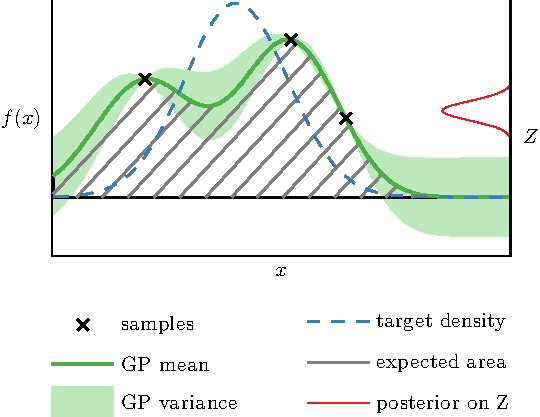
\includegraphics[width=\columnwidth]{figs/herding/bq_intro4}
\caption{An illustration of Bayesian Quadrature.  The function $f(x)$ is sampled at a set of input locations.  This induces a Gaussian process posterior distribution on $f$, which is integrated in closed form against the target density, $p(\vx)$.  Since the amount of volume under $f$ is uncertain, this gives rise to a (Gaussian) posterior distribution over $Z_{f,p}$.}
\label{fig:bq_intro}
\end{figure}

So far, we have only considered integration methods in which the integral \eqref{eqn:integral} is approximated by the empirical mean of the function evaluated at some set of samples, or pseudo-samples.  Equivalently, we can say that Monte Carlo and herding both assign an equal $\frac{1}{N}$ weight to each of the samples.

In \citep{BZMonteCarlo}, an alternate method is propositionosed: Bayesian Monte Carlo, or Bayesian quadrature (\bq).  \bq{} puts a prior distribution on $\vf$, then estimates integral \eqref{eqn:integral} by inferring a posterior distribution over the function $\vf$, conditioned on the observations $\vf(\vx_n)$ at some query points $\vx_n$.  The posterior distribution over $f$ then implies a distribution over $Z_{f,p}$.  This method allows us to choose sample locations $\vx_n$ in any desired manner. See Figure \ref{fig:bq_intro} for an illustration of Bayesian Quadrature.

%In \cite{BZMonteCarlo}, an alternate method was propositionosed: Bayesian Monte Carlo, or Bayesian quadrature (\bq).  \bq{} puts a prior distribution on $\vf$, then conditions on the observations $\vf(\vx_n)$ to obtain a posterior distribution over the function $\vf$.  The posterior over $\vf$ then implies a Then estimates integral \eqref{eqn:integral} by 


\subsubsection{ BQ Estimator}

Here we derive the \bq{} estimate of \eqref{eqn:integral}, after conditioning on function evaluations $\vf(\vx_1) \dots \vf(\vx_N)$, denoted as $f(\vX)$.  The Bayesian solution implies a distribution over $Z_{f,p}$.  The mean of this distribution, $\expect{}{Z}$ is the optimal Bayesian estimator for a squared loss.

For simplicity, $\vf$ is assigned a Gaussian process prior with kernel function $k$ and mean $0$.  This assumption is very similar to the one made by kernel herding in Eqn.\ \eqref{eq:mmd_assumption}.

After conditioning on $\vf_{\vx}$, we obtain a closed-form posterior over $\vf$:
%
\begin{align}
p(\vf(\vx\st)|\vf(\vX)) = \Normal{\vf_{\vx\st}}{\mf(\vx\st)}{\cov(\vx\st,\vx\st')}
\end{align} 
where
\begin{align}
\mf(\vx\st) = & k(\vx\st, \vX) K^{-1} \vf(\vX) \\
\cov(\vx\st, \vx\st') = & k(\vx\st,\vx\st) - k(\vx\st, \vX) K^{-1} k(\vX, \vx\st)
\end{align} 
%
and $K = k(\vX, \vX)$. 
%
Conveniently, the \gp{} posterior allows us to compute the expectation of \eqref{eqn:integral} in closed form: 
%
%\begin{align}
%Z & = \int f(\vx)p(\vx)d\vx
%\end{align} 
%so we integrate over functions to get:
\begin{align}
\expect{\gp}{Z} & = \expect{\gp}{\int f(\vx)p(\vx)d\vx}\\
 & = \int\!\!\! \int\!\! f(\vx) p(f(\vx)|\vf(\vX)) p(\vx) d\vx df\\
 & = \int\!\!\! \mf(\vx) p(\vx) d\vx \\
 & = \left[ \int\!\! k(\vx, \vX) p(\vx) d\vx \right] K^{-1} \vf(\vX) \\
 & = \vz^T K^{-1} \vf(\vX)
\label{eq:marg_mean_symbolic}
\end{align} 
where
\begin{align}
z_n & = \int\!\! k(\vx, \vx_n) p(\vx) d\vx = \expect{\vx' \sim p}{k(\vx_n, \vx')}.
\end{align}
%
Conveniently, as in kernel herding, the desired expectation of $Z_{f,p}$ is simply a linear combination of observed function values $\vf(\vx)$:
%
\begin{align}
\expect{\gp}{Z} & = \vz^T K^{-1} \vf(\vX) \\
    & = \sum_n w_{\bq}^{(n)} \vf_{\vx_n})
\end{align}  
where
\begin{align}  
w_{\bq}^{(n)} & = \sum_m \vz_j^T K^{-1}_{nm}
\label{eq:bq_weights}
\end{align}
%
Thus, we can view the BQ estimate as a weighted version of the herding estimate.  Interestingly, the weights $\vw_{\bq}$ do not need to sum to 1, and are not even necessarily positive.

\subsubsection{Non-normalized and Negative Weights}

\begin{figure}
\centering
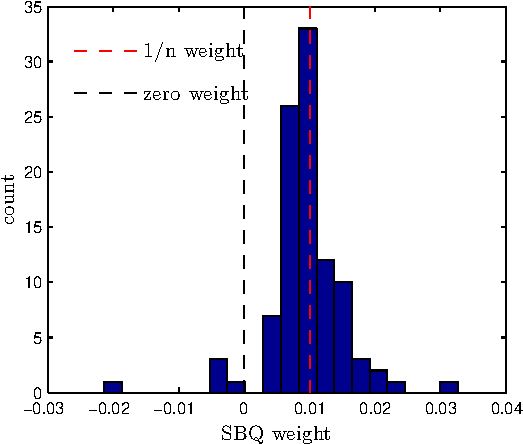
\includegraphics[width=\columnwidth]{figs/herding/weights_v1_n100}
\caption{A set of optimal weights given by \bq{}, after 100 \sbq{} samples were selected on the distribution shown in Figure \ref{fig:fig1}.  Note that the optimal weights are spread away from the uniform weight ($\frac{1}{N}$), and that some weights are even negative.  The sum of these weights is 0.93.}
\label{fig:weights100}
\end{figure}

When weighting samples, it is often assumed, or enforced \citep[as in][]{bach2012equivalence,Song2008}, that the weights $\vw$ form a probability distribution.  However, there is no technical reason for this requirement, and in fact, the optimal weights do not have this propositionerty.  Figure \ref{fig:weights100} shows a representative set of 100 \bq{} weights chosen on samples representing the distribution in figure \ref{fig:fig1}.  There are several negative weights, and the sum of all weights is 0.93.

Figure \ref{fig:weights_shrinkage} demonstrates that, in general, the sum of the Bayesian weights exhibits shrinkage when the number of samples is small.

\begin{figure}
\centering
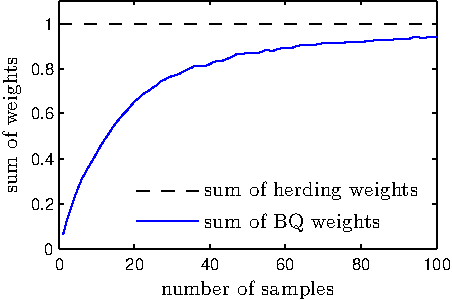
\includegraphics[width=\columnwidth]{figs/herding/weights_shrinkage}
\caption{An example of Bayesian shrinkage in the sample weights.  In this example, the kernel width is approximately $\nicefrac{1}{20}$ the width of the distribution being considered.  Because the prior over functions is zero mean, in the small sample case the weights are shrunk towards zero.  The weights given by simple Monte Carlo and herding do not exhibit shrinkage. }
\label{fig:weights_shrinkage}
\end{figure}

%For a fixed kernel, the variance of the BQ estimate does not depend on the function values.

%A natural criterion for selecting sample locations would be to choose locations which most reduce the variance of $Z_{f,p}$.

\subsubsection{Optimal sampling for BQ}

Bayesian quadrature provides not only a mean estimate of $Z_{f,p}$, but a full Gaussian posterior distribution. The variance of this distribution $\var{}{Z_{f,p}|f_{x_1}, \dots, f_{x_N}}$ quantifies our uncertainty in the estimate. When selecting locations to evaluate the function $f$, minimising the posterior variance is a sensible strategy. Below, we give a closed form formula for the posterior variance of $Z_{f,p}$, conditioned on the observations $f_{x_1} \dots f_{x_N}$, which we will denote by $\epsilon^2_{\bq{}}$.  For a longer derivation, see \cite{BZMonteCarlo}.
\begin{align}
\epsilon^{2}_{\bq{}}(\vx_1,\ldots,\vx_N) & = 
\var{}{Z_{f,p}|f_{x_1}, \dots, f_{x_N}} \\
% \nonumber & = \expect{f \sim \gp, p\sim p(x)}{ \left( f(\vx) - \mf(\vx) \right)\left( f(\vx') - \mf(\vx') \right)} \\ 
%\nonumber & = \int \Bigg( \!\! \left( \int f(\vx) p(\vx) d\vx - \int \mf(\vx') p(\vx') d\vx' \right) \\ 
%\nonumber & \quad \times \left( \int f(\vx) p(\vx) d\vx - \int \mf(\vx') p(\vx') d\vx' \right) \!\! \Bigg) p(f) df \\ 
%\nonumber & = \int\!\!\! \int\!\! \int\!\! \left[ f(\vx) - \mf(\vx) \right] \left[ f((\vx') - \mf(\vx') \right] p(f) df \\
%\nonumber & \qquad \times   p(\vx) p(\vx') d\vx d\vx' \\
%\nonumber & = \int\!\! \!\int\!\! \Cov \left[ f((\vx), f((\vx') \right] p(\vx) p(\vx') d\vx d\vx' \\
%\nonumber & = \int\!\!\! \int\!\! \left[ k(\vx, \vx') - k(\vx, \vX) K^{-1} k(\vX, \vx') \right] \\
%\nonumber          & \qquad \times p(\vx) p(\vx') d\vx d\vx' \\ 
%\nonumber & = \int\!\!\! \int\!\! k(\vx, \vx') p(\vx) p(\vx') d\vx d\vx' \\
%\nonumber & \quad - \left[ \int\!\! k(\vx, \vX) p(\vx) d\vx \right] K^{-1} \left[ \int\!\! k(\vX, \vx') p(\vx') d\vx' \right] \\
& = \expect{\vx, \vx' \sim p}{k(\vx, \vx')} - \vz^T K^{-1} \vz\mbox{,}
\label{eq:marg_var_symbolic}
\end{align}
where $\vz_n = \expect{\vx' \sim p}{k(\vx_n, \vx')}$ as before. Perhaps surprisingly, the posterior variance of $Z_{f,p}$ does not depend on the observed function values, only on the location $x_n$ of samples. A similar independence is observed in other optimal experimental design problems involving Gaussian processes \citep{guestrin1}. This allows the optimal samples to be computed ahead of time, before observing any values of $f$ at all \citep{minka2000dqr}.
%\begin{align}
%\epsilon^{2}_{\bq{}}(\vx_1,\ldots,\vx_N) = \expect{\vx, \vx' \sim p}{k(\vx, \vx')} - \vz^T K^{-1} \vz
%\end{align}

We can contrast the \bq{} objective $\epsilon^{2}_{\bq{}}$ in \eqref{eq:marg_var_symbolic} to the objective being minimized in herding, $\epsilon^{2}_{herding}$ of equation \eqref{eq:mmd_assumption}. Just like $\epsilon^{2}_{herding}$, $\epsilon^{2}_{\bq{}}$ expresses a trade-off between accuracy and diversity of samples. On the one hand, as samples get close to high density regions under $p$, the values in $\vz$ increase, which results in decreasing variance. On the other hand, as samples get closer to each other, eigenvalues of $K$ increase, resulting in an increase in variance. 

In a similar fashion to herding, we may use a greedy method to minimise $\epsilon^{2}_{\bq{}}$, adding one sample at a time. We will call this algorithm \emph{Sequential Bayesian Quadrature} (\sbq{}):
\begin{align}
\vx_{n+1} &\leftarrow \argmin_{\vx \in \mathcal{X}} \epsilon_{\bq{}}\left(\{\vx_1,\ldots,\vx_{n},\vx\}\right)
\end{align}
Using incremental updates to the Cholesky factor, the criterion can be evaluated in $\mathcal{O}(n^2)$ time. Iteratively selecting $N$ samples thus takes $\mathcal{O}(N^3)$ time, assuming optimisation can be done on $\mathcal{O}(1)$ time.

\subsubsection{RELATING $\var{}{Z_{f,p}}$ TO $\mmd$}

The similarity in the behaviour of $\epsilon^{2}_{herding}$ and $\epsilon^{2}_{\bq{}}$ is not a coincidence, the two quantities are closely related to each other, and to \mmd.
	
\begin{proposition} The expected variance in the Bayesian quadrature $\epsilon^{2}_{\bq{}}$  is the maximum mean discrepancy between the target distribution $p$ and $q_{\bq{}}(x) = \sum_{n=1}^{N}w^{(n)}_{\bq{}}\delta_{x_n}(x)$
\end{proposition}
%
\begin{proof}
The proof involves invoking the representer theorem, using bilinearity of scalar products and the fact that if $f$ is a standard Gaussian process then $\forall g\in\He: \left\langle f,g\right\rangle \sim \mathcal{N}(0,\Hnorm{g})$:
\begin{align}
&\var{}{Z_{f,p}\vert f_{x_1}, \dots, f_{x_N}}=\\
	&= \mathbb{E}_{f\sim GP} \left( \int f(x) p(x) dx - \sum_{n=1}^{N}w^{(n)}_{\bq{}} f(x_n)\right)^2\\
	&= \mathbb{E}_{f\sim GP} \left( \int \left\langle f, \phi (x)\right\rangle p(x) dx - \sum_{n=1}^{N}w^{(n)}_{\bq{}} \left\langle f, \phi (x_n)\right\rangle\right)^2\\
	&= \mathbb{E}_{f\sim GP} \left\langle f ,  \int\phi(x) p(x) dx - \sum_{n=1}^{N}w^{(n)}_{\bq{}}\phi(x_n)\right\rangle^2\\
	&= \Hnorm{\mu_p - \mu_{q_{\bq{}}}}^2\\
	&= \mmd^2(p,q_{\bq{}})
\end{align}
\end{proof}

We know that the the posterior mean $\expect{\gp}{Z_{f,p}\vert f_1,\ldots,f_N}$ is a Bayes estimator and has therefore the minimal expected squared error amongst all estimators. This allows us to further rewrite $\epsilon^{2}_{\bq{}}$ into the following minimax forms:
%
\begin{align}
\epsilon^{2}_{\bq{}} &= \sup_{\substack{f\in\He\\\Hnorm{f}{\He}=1}} \left| \int f_x p(x) dx - \sum_{n=1}^{N}w^{(n)}_{\bq{}} f_{x_n}\right|^2\\
	&= \inf_{\hat{Z}:\mathcal{X}^N\mapsto\mathbb{R}} \sup_{\substack{f\in\He\\\Hnorm{f}=1}} \left| Z - \hat{Z}\left(f_{x_1},\ldots,f_{x_N}\right)\right|^2\\
	&= \inf_{\bm{w}\in\mathbb{R}^N} \sup_{\substack{f\in\He\\\Hnorm{f}=1}} \left| \int f_x p(x) dx - \sum_{n=1}^{N}w_n 	f_{x_n}\right|^2
\end{align}
%
Looking at $\epsilon^{2}_{\bq{}}$  this way, we may discover the deep similarity to the criterion $\epsilon^2_{herding}$ that kernel herding minimises. Optimal sampling for Bayesian quadrature minimises the same objective as kernel herding, but with the uniform $\frac{1}{N}$ weights replaced by the optimal weights. As a corollary
%
\begin{align}
\epsilon^{2}_{\bq{}}(x_1,\ldots,x_N)  \leq \epsilon^{2}_{KH} (x_1,\ldots,x_N)
\end{align}

It is interesting that $\epsilon^{2}_{\bq{}}$ has both a Bayesian interpretation as posterior variance under a Gaussian process prior, and a frequentist interpretation as a minimax bound on estimation error with respect to an RKHS.

\subsubsection{SUBMODULARITY}

\label{sec:submodularity}

In this section, we use the concept of approximate submodularity \citep{KrauseCevher10}, in order to study convergence propositionerties of \sbq{}.

A set function $s:2^\mathcal{X} \mapsto \mathbb{R}$ is \textit{submodular} if, for all $A\subseteq B\subseteq \mathcal{X}$ and $\forall x \in \mathcal{X}$
%
\begin{align}
s(A\cup\{x\})-s(A)\geq s(B\cup\{x\})-s(B)
\end{align}
%
Intuitively, submodularity is a diminishing returns propositionerty: adding an element to a smaller set has larger relative effect than adding it to a larger set. A key result \cite[see e.\,g.\ ][and references therein]{KrauseCevher10} is that greedily maximising a submodular function is guaranteed not to differ from the optimal strategy by more than a constant factor of $(1-\frac{1}{e})$.

Herding and \sbq{} are examples of greedy algorithms optimising set functions: they add each pseudosample in such a way as to minimize the instantaneous reduction in $\mmd$. So it is intuitive to check whether the objective functions these methods minimise are submodular. Unfortunately, neither $\epsilon_{herding}$, not $\epsilon_{\bq{}}$ satisfies all conditions for submodularity. However, noting that \sbq{} is identical to the sparse dictionary selection problem studied in detail by \citet{KrauseCevher10}, we can conclude that \sbq{} satisfies a weaker condition called \emph{approximate submodularity}. 

A set function $s:2^\mathcal{X} \mapsto \mathbb{R}$ is \textit{approximately submodular} with constant $\epsilon>0$, if for all $A\subseteq B\subseteq \mathcal{X}$ and $\forall x \in \mathcal{X}$
%
\begin{align}
s(A\cup\{x\})-s(A)\geq s(B\cup\{x\})-s(B) - \epsilon
\end{align}

\begin{proposition}\label{proposition:submodularity_SBQ}
$\epsilon^{2}_{\bq{}}(\emptyset)-\epsilon^{2}_{\bq{}}(\cdot)$ is weakly a weakly submodular set function with constant $\epsilon<4r$, where $r$ is the incoherency
\begin{equation}
	r = \max_{x,x'\in\mathcal{P}\subseteq\mathcal{X}} \frac{k(x,x')}{\sqrt{k(x,x)k(x',x')}}
\end{equation}
\end{proposition}
\begin{proof} By the definition of $\mmd$ we can see that
$-\epsilon^{2}_{\bq{}} = \inf_{w\in\mathbb{R}^N}\Hnorm{\mu_p - \sum_{n=1}^N w^{(n)}_{\bq{}}k(\cdot,\vx_n)}^2$ is the negative squared distance between the mean element $\mu_p$ and its projection onto the subspace spanned by the elements $k(\cdot,\vx_n)$. Substituting $k=1$ into Theorem 1 of \citet{KrauseCevher10} concludes the proof.
\end{proof}

Unfortunately, weak submodularity does not provide the strong near-optimality guarantees as submodularity does . If $s:2^\mathcal{X} \mapsto \mathbb{R}$ is a weakly submodular function with constant $\epsilon$, and $\vert\mathcal{A}_n\vert=n$ is the result of greedy optimisation of $s$, then
\begin{equation}
	s(\mathcal{A}_n) \geq \left(1-\frac{1}{e}\right)\max_{\vert\mathcal{A}\vert\leq n}s(\mathcal{A}) - n\epsilon
\end{equation}

As pointed out by \citet{KrauseCevher10}, this guarantee is very weak as in our case the objective function $\epsilon^{2}_{\bq{}}(\emptyset)-\epsilon^{2}_{\bq{}}(\cdot)$ is upper bounded by a constant. However, establishing a connection between \sbq{} and sparse dictionary selection problem opens up interesting directions for future research, and it may be possible to apply algorithms and theory developed for sparse dictionary selection to kernel-based quasi-Monte Carlo methods.

\subsubsection{EXPERIMENTS}
\label{sec:experiments}

In this section, we examine empirically the rates of convergence of sequential Bayesian quadrature and herding.  We examine both the expected error rates, and the empirical error rates.

In all experiments, the target distribution $p$ is chosen a 2D mixture of 20 Gaussians, whose equiprobability contours are shown in Figure \ref{fig:fig1}. To ensure a comparison fair to herding, the target distribution, and the kernel used by both methods, correspond exactly to the one used in \citep[Fig. 1]{chen2010super}. %Herding and \sbq{} used identical kernels for all experiments.
%
For experimental simplicity, each of the sequential sampling algorithms minimizes the next sample location from a pool of 10000 locations randomly drawn from the base distribution. In practice, one would run a local optimizer from each of these candidate locations, however in our experiments we found that this did not make a significant difference in the sample locations chosen. 

\subsubsection{Matching a distribution}

We first extend an experiment from \citep{chen2010super} designed to illustrate the mode-seeking behavior of herding in comparison to random samples. In that experiment, %e first experiment of \cite{chen2010super}, 
it is shown that a small number of i.\,i.\,d.\ samples drawn from a multimodal distribution will tend to, by chance, assign too many samples to some modes, and too few to some other modes. In contrast, herding places `super-samples' in such a way as to avoid regions already well-represented, and seeks modes that are under-represented.

We demonstrate that although herding improves upon i.\,i.\,d.\ sampling, the uniform weighting of super-samples leads to sub-optimal performance.  Figure \ref{fig:fig1} shows the first 20 samples chosen by kernel herding, in comparison with the first 8 samples chosen by \sbq{}.  By weighting the 8 \sbq{} samples by the quadrature weights in \eqref{eq:bq_weights}, we can obtain the same expected loss as by using the 20 uniformly-weighted herding samples.  
%
\begin{figure}
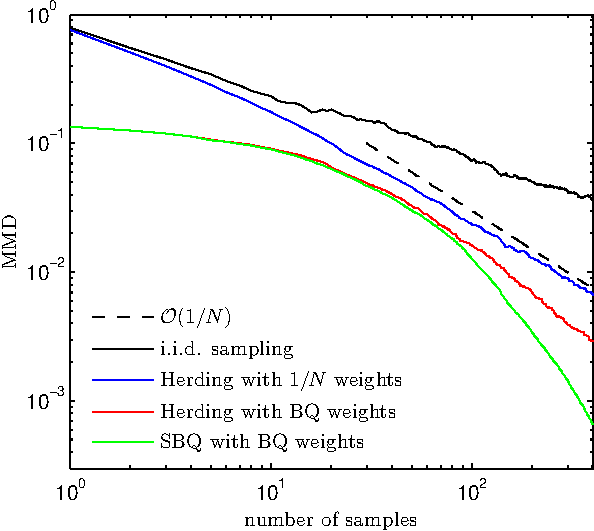
\includegraphics[width=\columnwidth]{figs/herding/expected_variance_v7_400}
\caption{The maximum mean discrepancy, or expected error of several different quadrature methods.  Herding appears to approach a rate close to $\mathcal{O}(1/N)$.  \sbq{} appears to attain a faster, but unknown rate.}
\label{fig:mmd_curve}
\end{figure}
%
Figure \ref{fig:mmd_curve} shows MMD versus the number of samples added, on the distribution shown in Figure \ref{fig:fig1}.  We can see that in all cases, \sbq{} dominates herding.  It appears that \sbq{} converges at a faster rate than $\mathcal{O}(1/N)$, although the form of this rate is unknown.

There are two differences between herding and \sbq{}:  \sbq{} chooses samples according to a different criterion, and also weights those samples differently.  We may ask whether the sample locations or the weights are contributing more to the faster convergence of \sbq{}. Indeed, in Figure \ref{fig:fig1} we observe that the samples selected by \sbq{} are quite similar to the samples selected by kernel herding. To answer this question, we also plot in Figure \ref{fig:mmd_curve} the performance of a fourth method, which selects samples using herding, but later re-weights the herding samples with \bq{} weights.  Initially, this method attains similar performance to \sbq{}, but as the number of samples increases, \sbq{} attains a better rate of convergence.  This result indicates that the different sample locations chosen by \sbq{}, and not only the optimal weights, are responsible for the increased convergence rate of \sbq{}.

\subsubsection{Estimating Integrals}

%\subsubsection{Functions in the RKHS}

We then examined the empirical performance of the different estimators at estimating integrals of real functions.  To begin with, we looked at performance on 100 randomly drawn functions, of the form:
%
\begin{align}
f(\vx) & = \sum_{i=1}^{10} \alpha_i k(\vx, \vc_i)
\end{align}
%
where
\begin{align}
\Hnorm{f}^2 = \sum_{i=1}^{10} \sum_{j=1}^{10} \alpha_i \alpha_j k(\vc_i, \vc_j) = 1
\end{align}
%
That is, these functions belonged exactly to the unit ball of the RKHS defined by the kernel $k(\vx, \vx')$ used to model them.
%
\begin{figure}
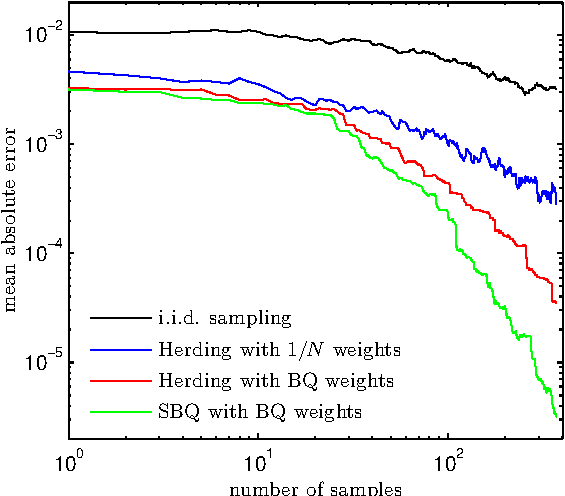
\includegraphics[width=\columnwidth]{figs/herding/error_curve_rkhs_400_v4}
\caption{Within-model error: The empirical error rate in estimating $Z_{f,p}$, for several different sampling methods, averaged over 250 functions randomly drawn from the RKHS corresponding to the kernel used.}
\label{fig:error_curve}
\end{figure}
%
Figure \ref{fig:error_curve} shows the empirical error versus the number of samples, on the distribution shown in Figure \ref{fig:fig1}.  The empirical rates attained by the method appear to be similar to the MMD rates in Figure \ref{fig:mmd_curve}.

By definition, MMD provides a upper bound on the estimation error in the integral of any function in the unit ball of the RKHS (Eqn.\ \eqref{eqn:rkhs-mmd}), including the Bayesian estimator, \sbq{}. Figure \ref{fig:bound_curve} demonstrates this quickly decreasing bound on the \sbq{} empirical error.

\begin{figure}
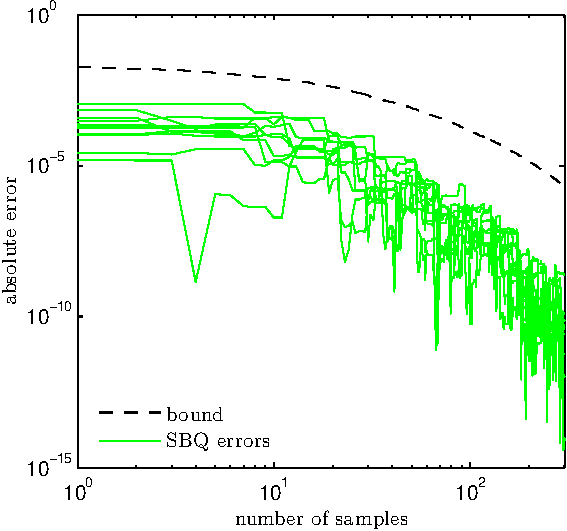
\includegraphics[width=\columnwidth]{figs/herding/bound_curve_rkhs}
\caption{The empirical error rate in estimating $Z_{f,p}$,  for the \sbq{} estimator, on 10 random functions drawn from the RKHS corresponding to the kernel used.  Also shown is the upper bound on the error rate implied by the $\mmd$.}
\label{fig:bound_curve}
\end{figure}

\subsubsection{Out-of-model performance}

A central assumption underlying \sbq{} is that the integrand function belongs to the RKHS specified by the kernel.  To see how performance is effected if this assumption is violated, we performed empirical tests with functions chosen from outside the RKHS.  We drew 100 functions of the form:
%
\begin{align}
f(\vx) & = \sum_{i=1}^{10} \alpha_i \exp(-\frac{1}{2} (\vx -\vc_i)^T \Sigma_i^{-1} (\vx -\vc_i)
\end{align}
%
where each $\alpha_i$ $\vc_i$ $\Sigma_i$ were drawn from broad distributions.  This ensured that the drawn functions had features such as narrow bumps and ridges which would not be well modelled by functions belonging to the isotropic kernel defined by $k$.
%
\begin{figure}
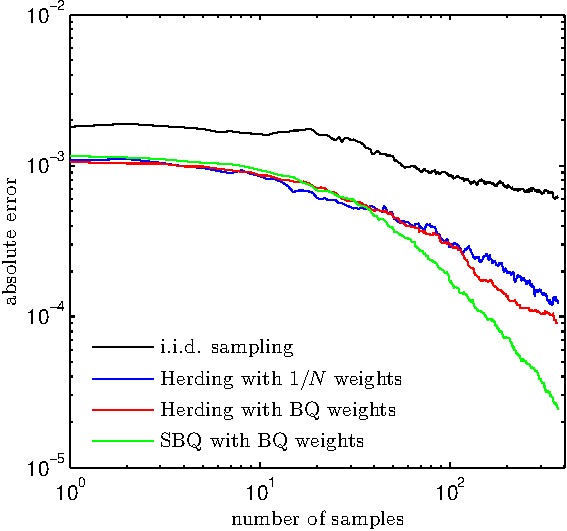
\includegraphics[width=\columnwidth]{figs/herding/error_curve_outmodel_400_v3}
\caption{Out-of-model error: The empirical error rates in estimating $Z_{f,p}$, for several different sampling methods, averaged over 250 functions drawn from outside the RKHS corresponding to the kernels used.}
\label{fig:error_curve_outmodel}
\end{figure}
%
Figure \ref{fig:error_curve_outmodel} shows that, on functions drawn from outside the assumed RKHS, relative performance of all methods remains similar.

Code to reproduce all results is available at \texttt{http://mlg.eng.cam.ac.uk/duvenaud/}

\subsubsection{DISCUSSION}

\subsubsection{Choice of Kernel}

Using herding techniques, we are able to achieve fast convergence on a Hilbert space of \emph{well-behaved} functions, but this fast convergence is at the expense of the estimate not necessarily converging for functions outside this space.
If we use a characteristic kernel \citep{Sriperumbudur2010}, such as the exponentiated-quadratic or Laplacian kernels, then convergence in MMD implies weak convergence of $q_N$ to the target distribution. 
%$p$\footnote{this statement is analogous to Levy's continuity theorem [cite], and we plan to include a more precise theorem and proof of this in the final version of the paper and supplementary material}. 
This means that the estimate converges for any bounded measurable function $f$. The speed of convergence, however, may not be as fast.

Therefore it is crucial that the kernel we choose is representative of the function or functions $f$ we will integrate.  For example, in our experiments, the convergence of herding was sensitive to the width of the Gaussian kernel.  One of the major weaknesses of kernel methods in general is the difficulty of setting kernel parameters.  A key benefit of the Bayesian interpretation of herding and MMD presented in this paper is that it provides a recipe for adapting the Hilbert space to the observations $f(x_n)$.  To be precise, we can fit the kernel parameters by maximizing the marginal likelihood of Gaussian process conditioned on the observations.  Details can be found in \citep{rasmussen38gaussian}.

\subsubsection{Computational Complexity}

While we have shown that Bayesian Quadrature provides the optimal re-weighting of samples, computing the optimal weights comes at an increased computational cost relative to herding. 
%
The computational complexity of computing Bayesian quadrature weights for $N$ samples is $\mathcal{O}(N^3)$, due to the necessity of inverting the Gram matrix $K(\vx, \vx)$.  Using the Woodbury identity, the cost of adding a new sample to an existing set is $\mathcal{O}(N^2)$.  For herding, the computational complexity of evaluating a new sample is only $\mathcal{O}(N)$, making the cost of choosing $N$ herding samples $\mathcal{O}(N^2)$.  For Monte Carlo, the cost of adding an i.i.d. sample from the target distribution is only $\mathcal{O}(1)$.

The relative computational cost of computing samples and weights using \bq{}, herding, and sampling must be weighed against the cost of evaluating $f$ at the sample locations.  Depending on this trade-off, the three sampling methods form a Pareto frontier over computational speed and estimator accuracy.  When computing $f$ is cheap, we may wish to use Monte Carlo methods.  In cases where $f$ is computationally costly, we would expect to choose the \sbq{} method.  When $f$ is relatively expensive, but a very large number of samples are required, we may choose to use kernel herding instead.  However, because the rate of convergence of \sbq{} is faster, there may be situations in which the $\mathcal{O}(N^3)$ cost is relatively inexpensive, due to the smaller $N$ required by \sbq{} to achieve the same accuracy as compared to using other methods.  

There also exists the possibility to switch to a less costly sampling algorithm as the number of samples increases.
%
\begin{table*}[t]
\begin{center}
\begin{tabular}{c|ccc}
%\hline
method & complexity & rate & guarantee\\
%\hline
\midrule
MCMC & $\mathcal{O}(N)$ & variable & ergodic theorem\\
i.i.d. MC & $\mathcal{O}(N)$ & $\frac{1}{\sqrt{N}}$ & law of large numbers\\
herding & $\mathcal{O}(N^2)$ & $\frac{1}{\sqrt{N}} \geq \cdot \geq \frac{1}{N}$ & \citep{chen2010super,bach2012equivalence} \\
SBQ & $\mathcal{O}(N^3)$ & unknown & approximate submodularity\\
%\hline
\end{tabular}
\end{center}
\caption{A comparison of the rates of convergence and computational complexity of several integration methods.}
\label{tbl:rates}
\end{table*}
%
Table \ref{tbl:rates} summarizes the rates of convergence of all the methods considered here.

\section{CONCLUSIONS}

In this paper, we have shown two main results:  First, we proved that the loss minimized by kernel herding is closely related to the loss minimized by Bayesian quadrature, when selecting sample locations. This implies that sequential Bayesian quadrature can viewed as an optimally-weighted version of kernel herding.

Second, we showed that the loss minimized by the Bayesian method is approximately submodular with respect to the samples chosen, and established connections to the submodular dictionary selection problem studied in \citep{KrauseCevher10}.

Finally, we empirically demonstrated a superior rate of convergence of \sbq{} over herding, and demonstrated a bound on the empirical error of the Bayesian quadrature estimate.

\subsubsection{Future Work}

In section \ref{sec:submodularity}, we showed that \sbq{} is approximately submodular, which provides only weak sub-optimality guarantees of its performance. It would be of interest to further explore the connection between Bayesian Quadrature and the dictionary selection problem to see if algorithms developed for dictionary selection can provide further practical or theoretical developments. The results in section \ref{sec:experiments}, specifically Figure \ref{fig:mmd_curve}, suggest that the convergence rate of \sbq{} is faster than $\mathcal{O}(1/N)$. However, we are not aware of any work showing what the theoretically optimal rate is. It would be of great interest to determine this optimal rate of convergence for particular classes of kernels.

\subsubsection*{Acknowledgements}

%The authors would like to thank Carl Rasmussen for helpful discussions, and Yutian Chen for his help in reproducing experiments.

%\appendix
%\section{Lemma on submodularity	}
%\label{app:submo}
%
%\begin{lem}\label{lemma:submodular}
%Let $\Pi_A$ be the operator that projects any vector to the subspace $S(A)$ spanned by a set of elements $A\subseteq\He$. For a fixed vector $p\in\He$, the following set-function $f_{p}(A):2^\He\mapsto\mathcal{R^{-}}$ is non-decreasing and submodular:
%\begin{align}
%f_{p}(A) = -\Hnorm{p-\Pi_{A}p}^2
%\end{align}
%\end{lem}
%\begin{proof}
%Submodularity of $f_p$ means that $\forall A\subseteq B\subseteq\He$ and $x\notin B$:
%\begin{align}
%	f_{p}(A\cup\{x\}) - f_{p}(A) \stackrel{?}{\geq} f_{p}(B\cup\{x\}) - f_{p}(B)
%\end{align}
%Spelling out the two quantities we get
%\begin{align}
%	-\Hnorm{p-\Pi_{A\cup\{x\}}p}^2 +\Hnorm{p-\Pi_{A}p}^2 \stackrel{?}{\geq}\\
%	 -\Hnorm{p-\Pi_{B\cup\{x\}}p}^2 +\Hnorm{p-\Pi_{B}p}^2
%\end{align}
%Using the Pythagorean theorem on both sides we get
%\begin{align}
%	-\Hnorm{\Pi_{A\cup\{x\}}p - \Pi_{A}p}^2 \stackrel{?}{\geq} -\Hnorm{\Pi_{B\cup\{x\}}p - \Pi_{B}p}^2
%\end{align}
%We can use the following Pythagorean identities
%\begin{align}
%	&\Hnorm{\Pi_{B\cup\{x\}}p - \Pi_{A}p}^2  =\\
%	 	&= \Hnorm{\Pi_{B\cup\{x\}}p - \Pi_{A\cup\{x\}}p}^2  + \Hnorm{\Pi_{A\cup\{x\}}p - \Pi_{A}p}^2 \\	
%	&\Hnorm{\Pi_{B\cup\{x\}}p - \Pi_{A}p}^2 = \\
%	&= \Hnorm{\Pi_{B\cup\{x\}}p - \Pi_{B}p}^2  + \Hnorm{\Pi_{B}p - \Pi_{A}p}^2 
%\end{align}
%Then our inequality becomes
%\begin{align}
%	\Hnorm{\Pi_{B\cup\{x\}}p - \Pi_{A\cup\{x\}}p}^2 \stackrel{?}{\geq} \Hnorm{\Pi_{B}p - \Pi_{A}p}^2
%\end{align}
%W.\,l.\,o.\,g.\ we can assume that $x\perp S(B)$, in which case using that
%\begin{align}
%\Pi_{B}\Pi_{B\cup\{x\}} &= \Pi_{B}\\
%\Pi_{B}\Pi_{A\cup\{x\}} &= \Pi_{A}\mbox{,}
%\end{align}
%we can write
%\begin{align}
%	\Hnorm{\Pi_{B\cup\{x\}}p - \Pi_{A\cup\{x\}}p}^2 \geq \Hnorm{\Pi_{B}\left(\Pi_{B\cup\{x\}}p - \Pi_{A\cup\{x\}}\right)}^2
%\end{align}
%Which is always true, as a projection of vectors is never longer than the vector itself.
%\end{proof}
%
%\pagebreak
\bibliographystyle{icml2012}
\bibliography{herding}

\end{document} 
